\section{Sekvensdiagrammer}

\subsection{Sekvensdiagrammer til UC's}

%Use case 2
\begin{figure}[H]
	\centering
	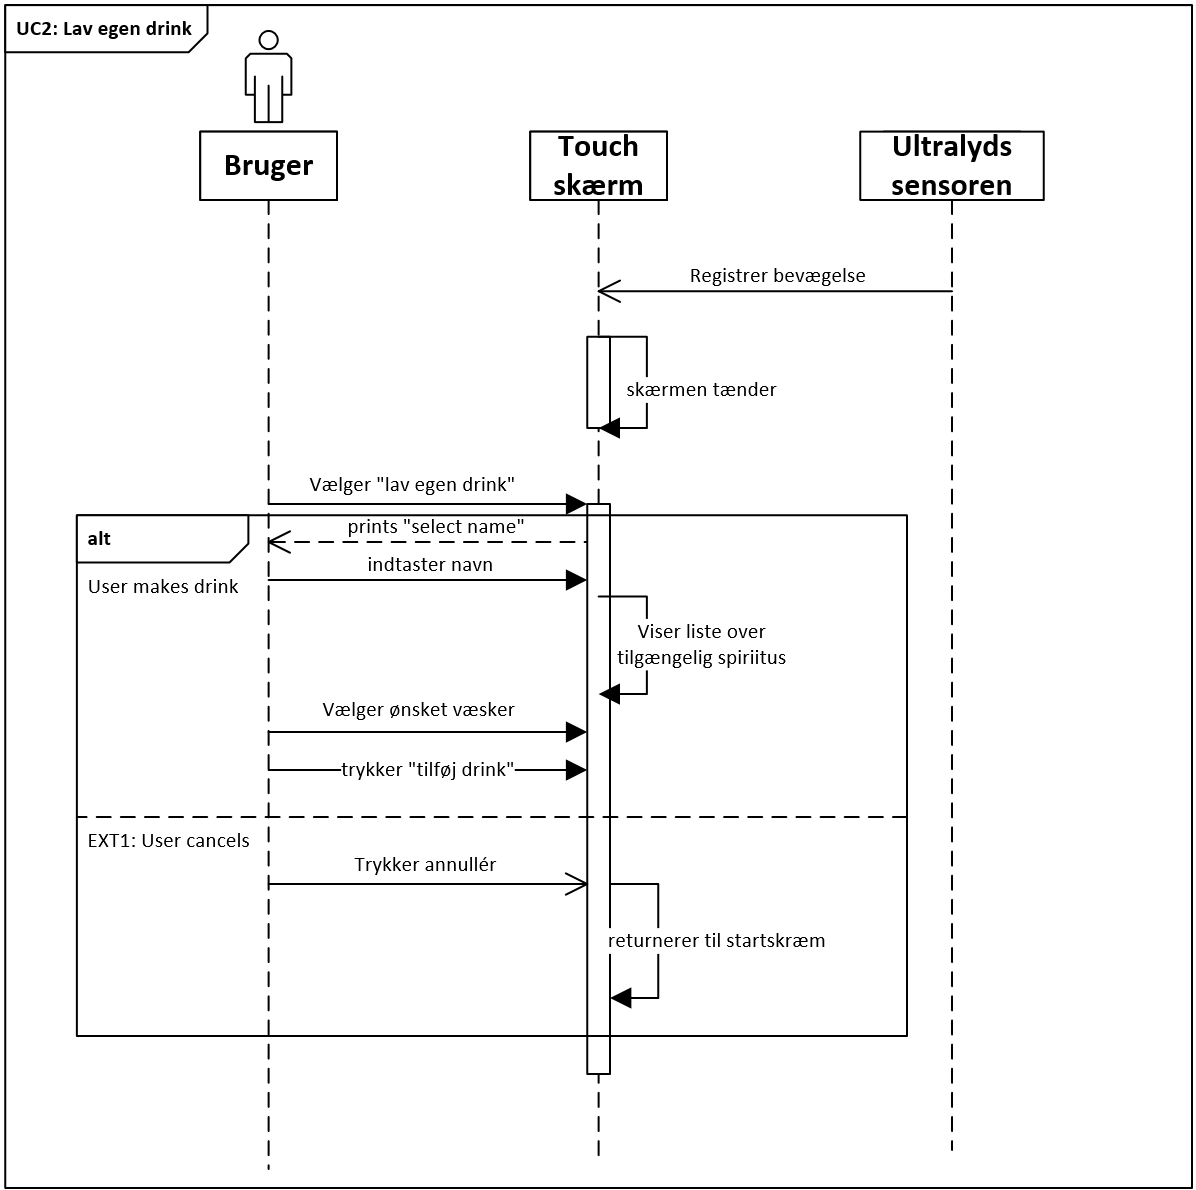
\includegraphics[width=1\textwidth]{Images/UC2lavegendrink.png}
	\caption{Sekvensdiagram for UC2: Lav egen drink}
	\label{fig:UC2}
\end{figure}

%Use case 3
\begin{figure}[H]
	\centering
	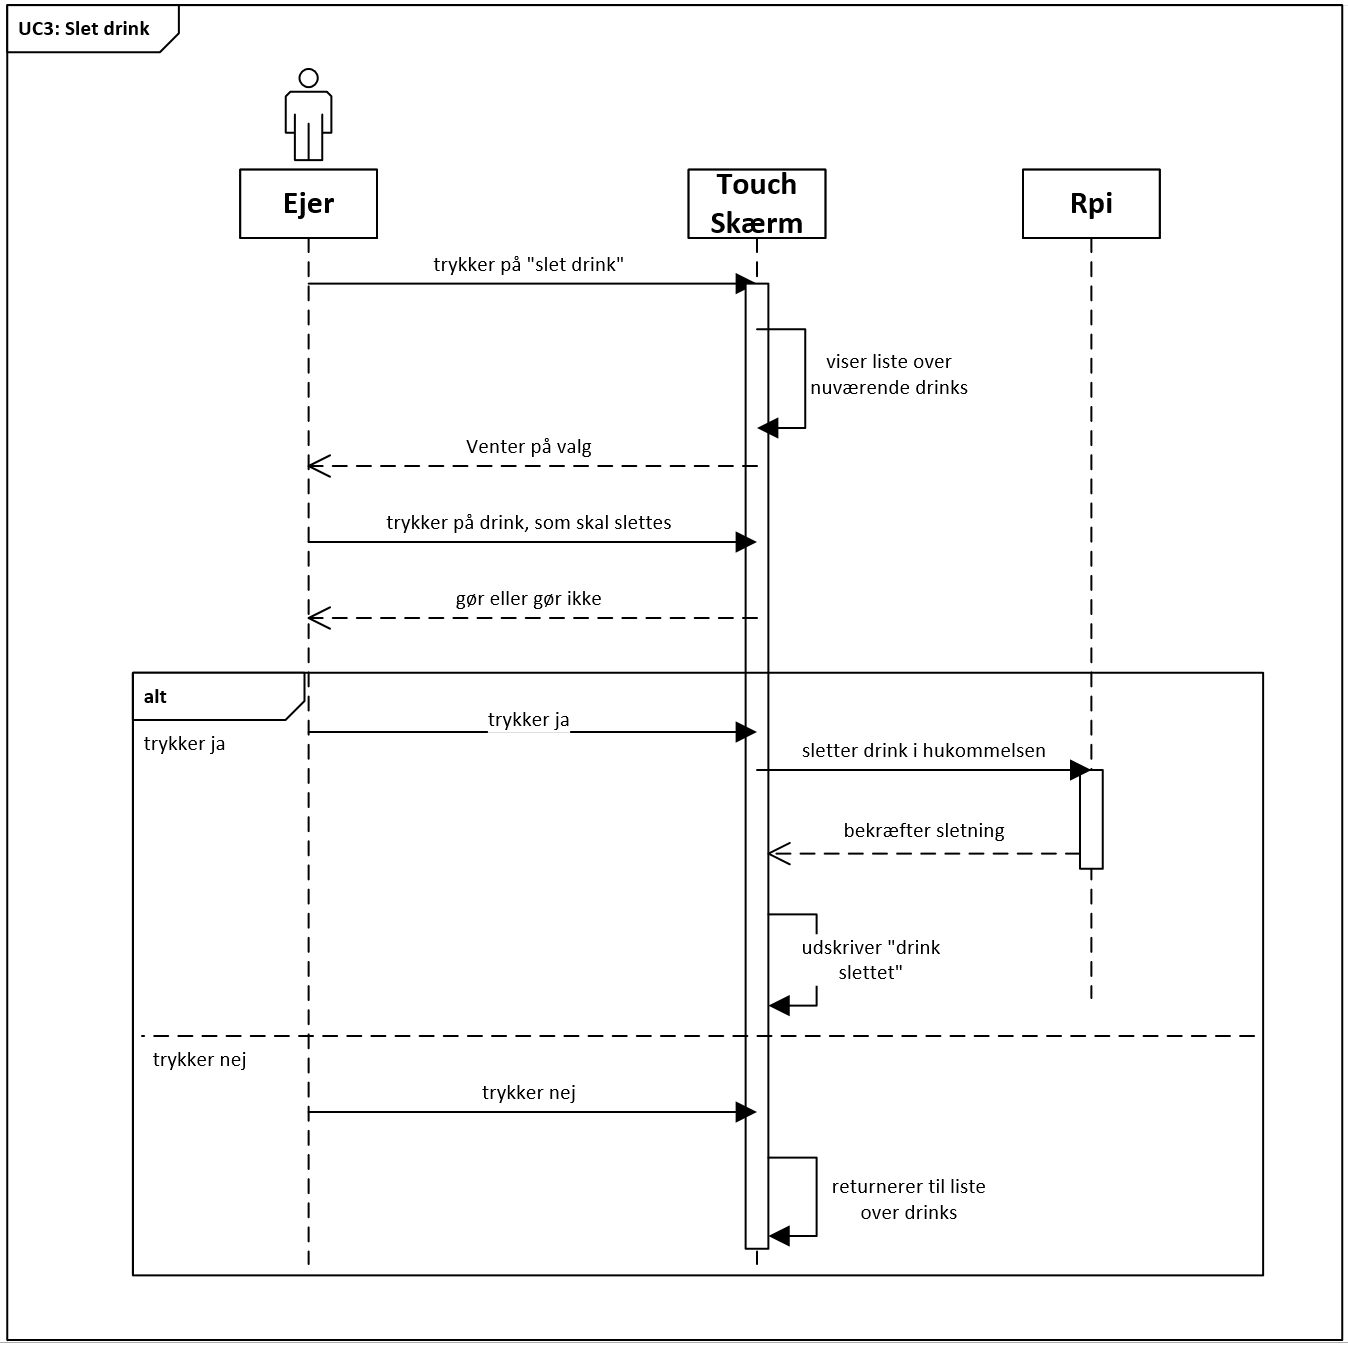
\includegraphics[width=1\textwidth]{Images/UC3sletdrink.png}
	\caption{Sekvensdiagram for UC3: Slet Drink}
	\label{fig:UC3}
\end{figure}

%Use case 4
\begin{figure}[H]
	\centering
	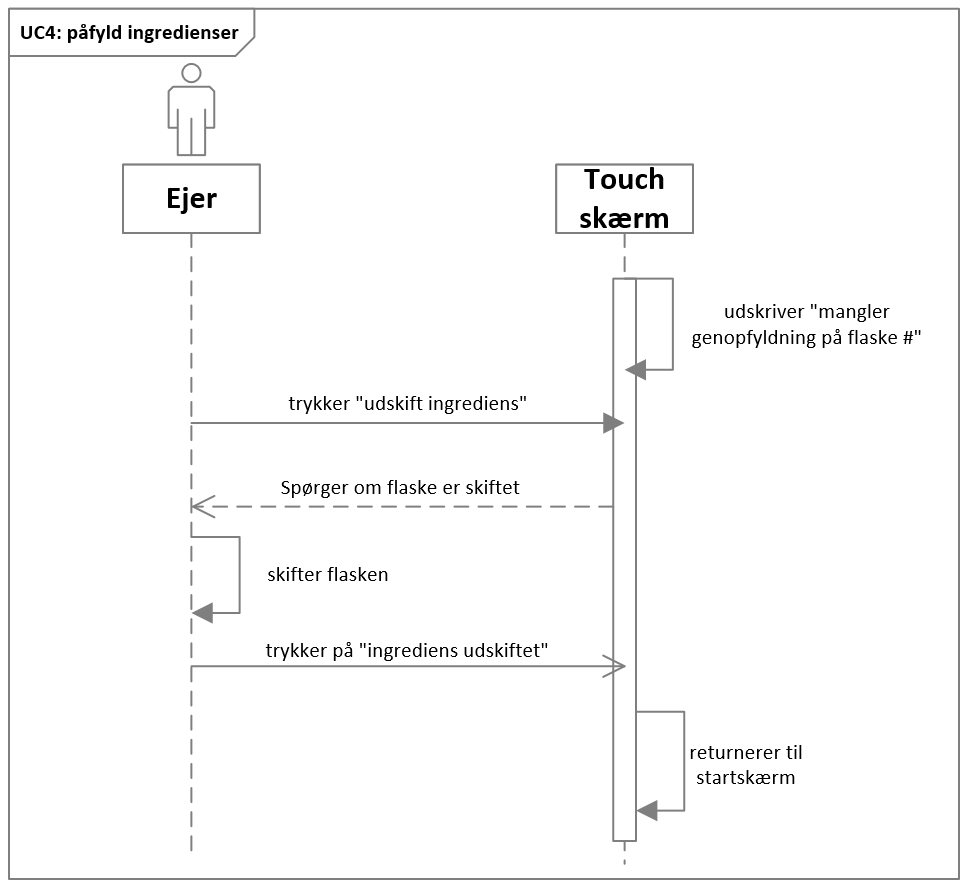
\includegraphics[width=1\textwidth]{Images/UC4paafyldingredienser.png}
	\caption{Sekvensdiagram for UC4: Påfyld ingredienser}
	\label{fig:UC4}
\end{figure}

%Use case 5
\begin{figure}[H]
	\centering
	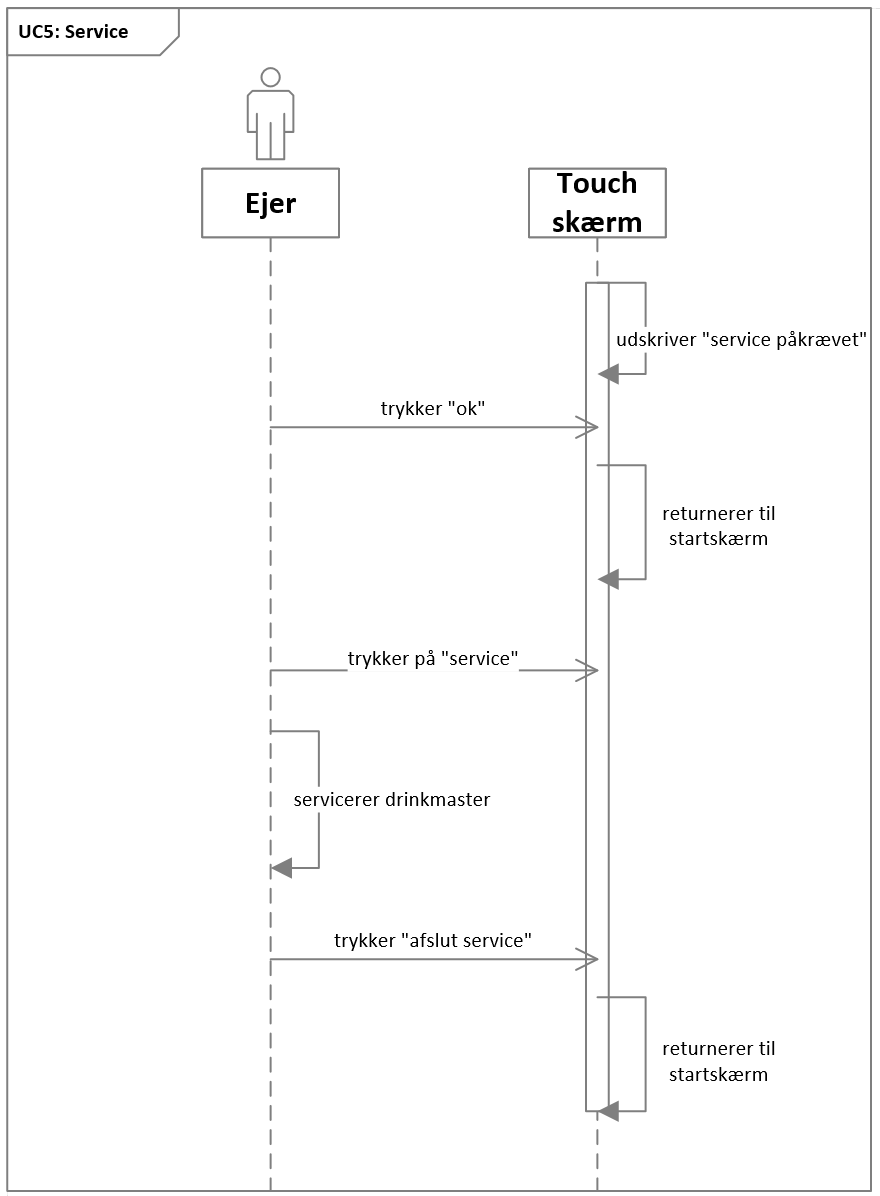
\includegraphics[width=1\textwidth]{Images/UC5service.png}
	\caption{Sekvensdiagram for UC5: Service}
	\label{fig:UC2_service}
\end{figure}

\subsection{Sekvensdiagrammer til test use cases}
%Test use case sekvensdiagrammer

\begin{figure}[H]
	\centering
	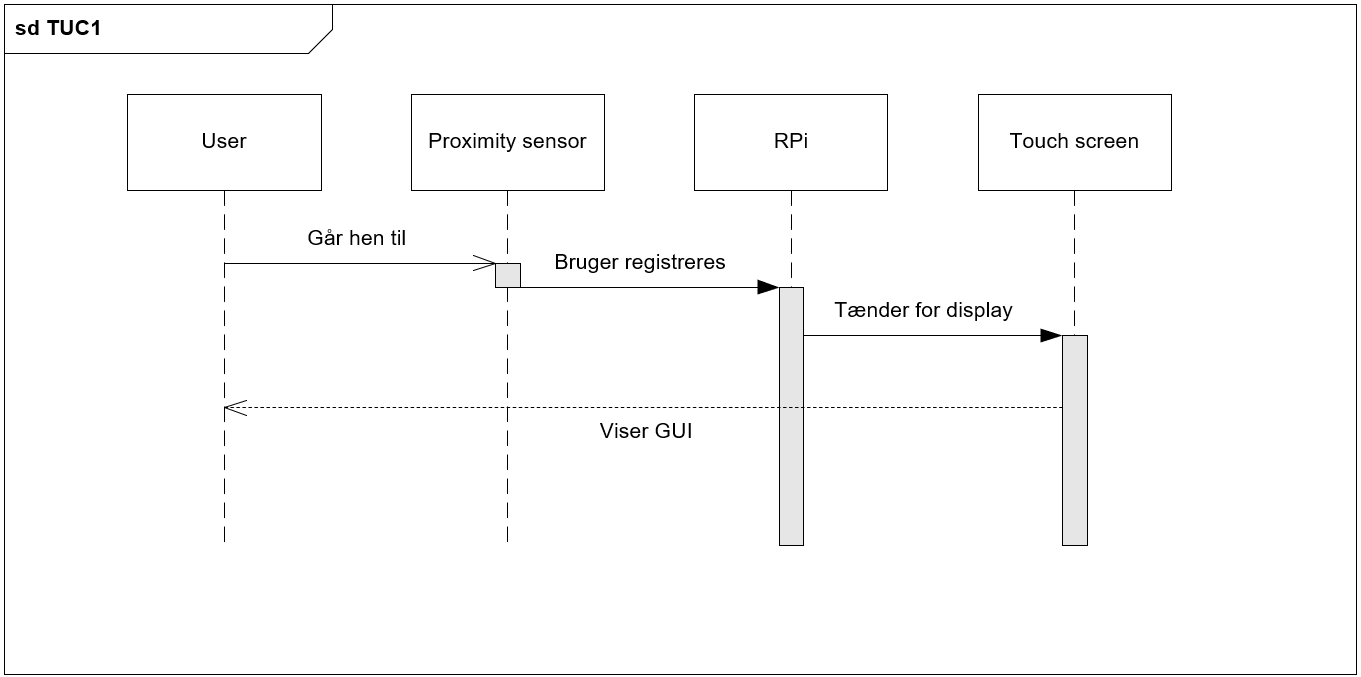
\includegraphics[width=1\textwidth]{Images/TUC1.png}
	\caption{Sekvensdiagram for test UC1: Registrer bruger}
	\label{fig:testUC1}
\end{figure}

\begin{figure}[H]
	\centering
	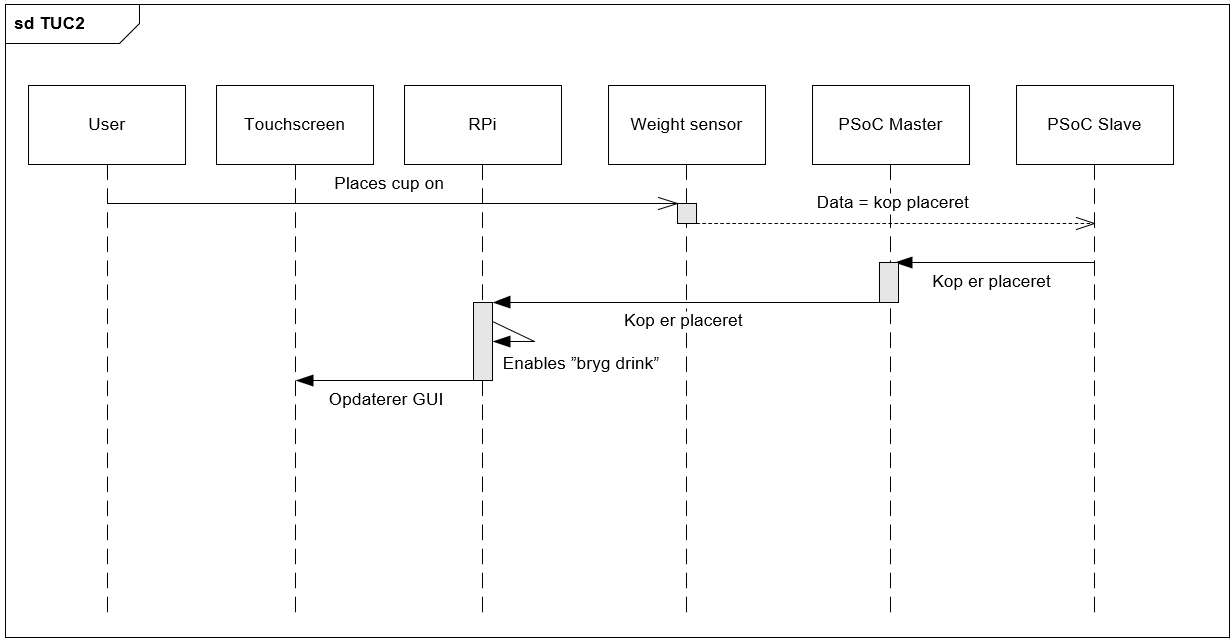
\includegraphics[width=1\textwidth]{Images/TUC2.png}
	\caption{Sekvensdiagram for test UC2: Vægt registrerer kop}
	\label{fig:testUC2}
\end{figure}

\begin{figure}[H]
	\centering
	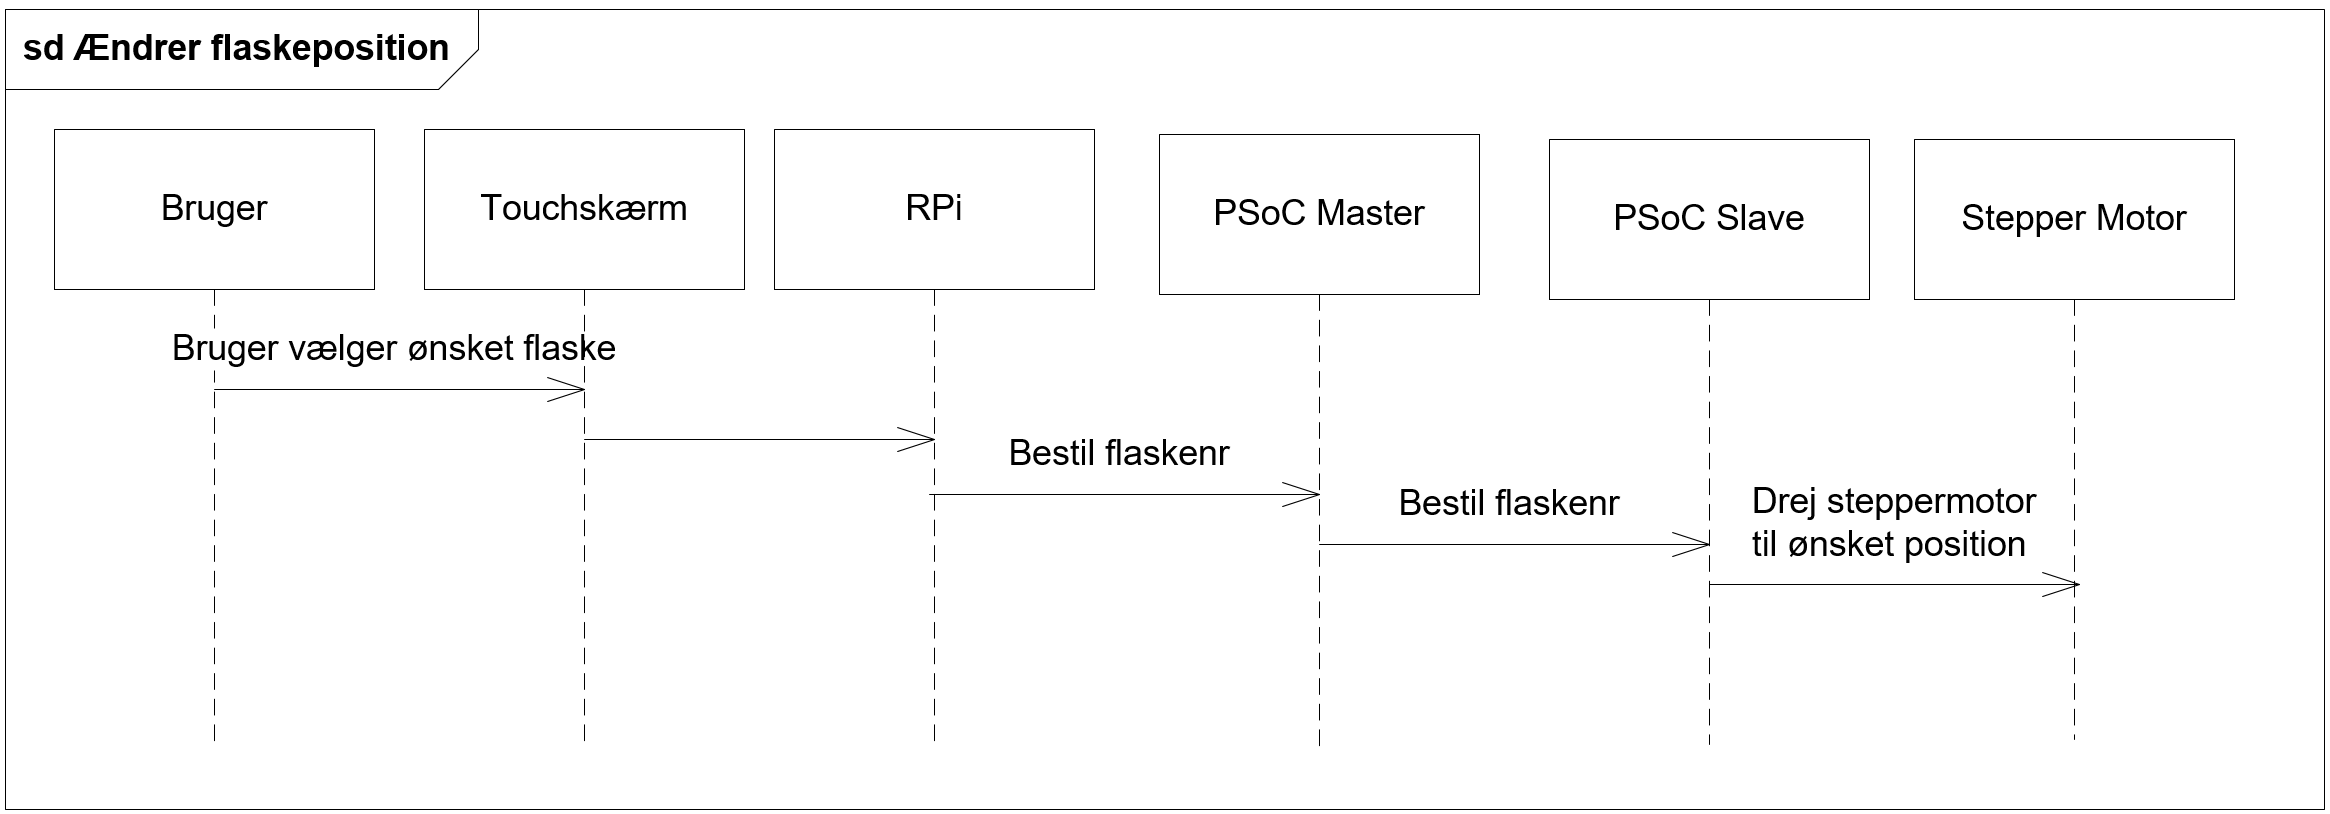
\includegraphics[width=1\textwidth]{Images/sdTestUC3.png}
	\caption{Sekvensdiagram for test UC3: Ændrer flaskeposition}
	\label{fig:testUC3}
\end{figure}

\begin{figure}[H]
	\centering
	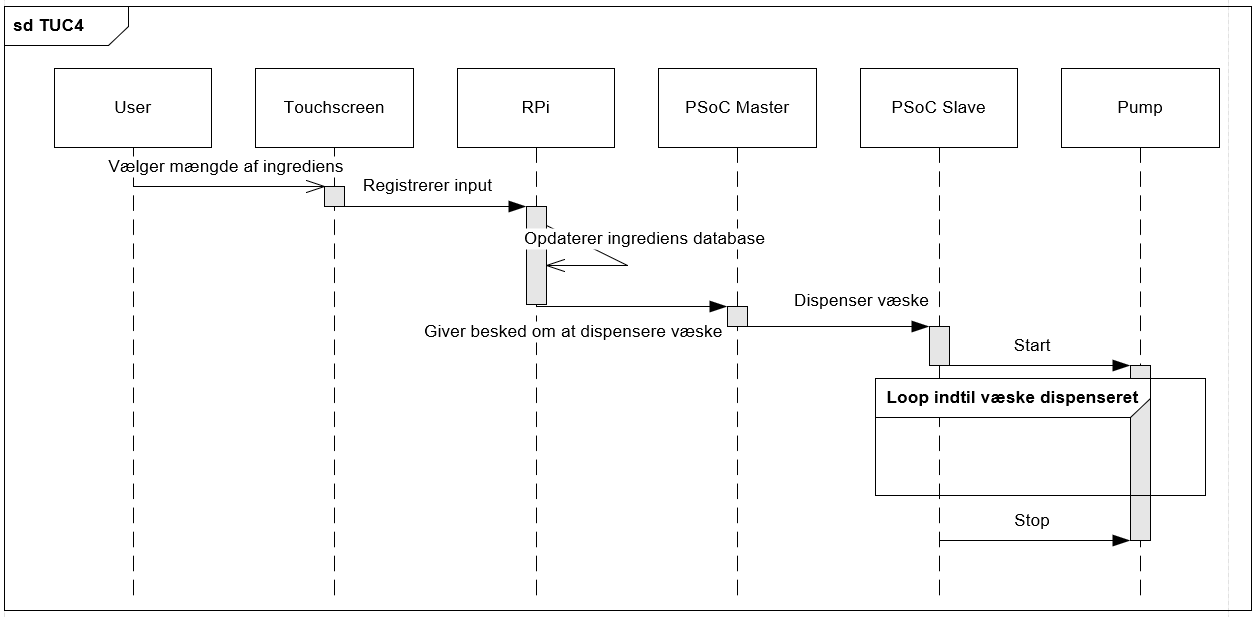
\includegraphics[width=1\textwidth]{Images/TUC4.png}
	\caption{Sekvensdiagram for test UC4: Doser væske}
	\label{fig:testUC4}
\end{figure}
\begin{figure}[H]
	\centering
	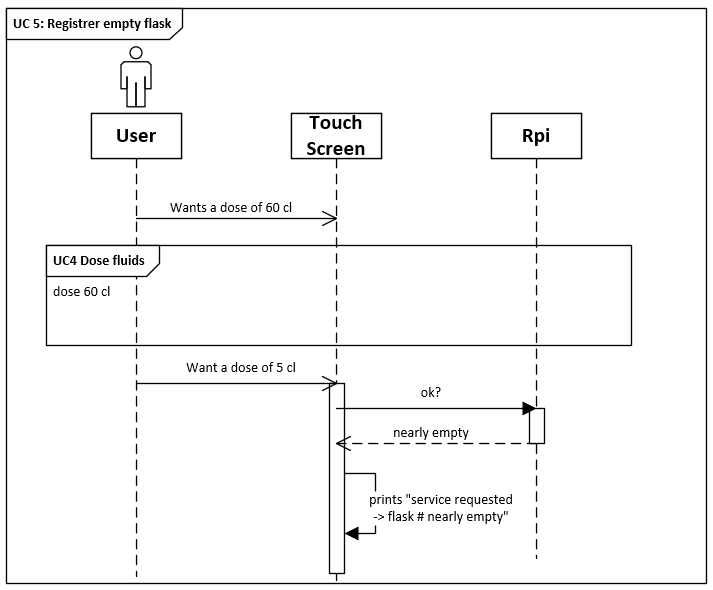
\includegraphics[width=1\textwidth]{Images/testUC5.png}
	\caption{Sekvensdiagram for test UC5: Registrer tom flaske}
	\label{fig:testUC5}
\end{figure}

\begin{figure}[H]
    \centering
    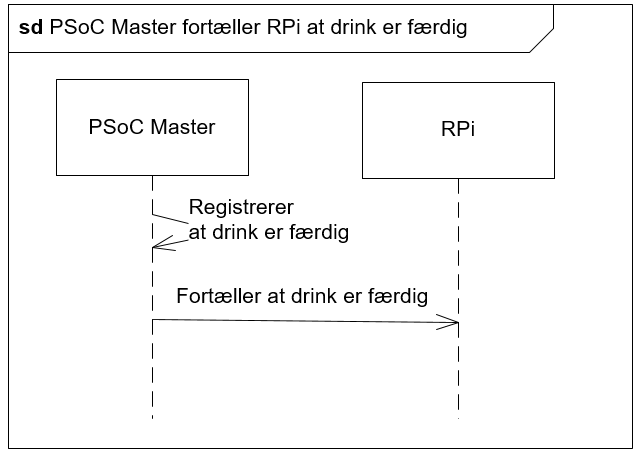
\includegraphics[width=1\textwidth]{Images/sdTestUC6.png}
    \caption{PSoC Master fortæller RPi at drink er færdig}
    \label{fig:testUC6}
\end{figure}